\documentclass[11pt,a4paper]{article}
\usepackage[T1]{fontenc}
\usepackage[latin1]{inputenc}
\usepackage{lmodern}
\usepackage{a4wide}
\usepackage[dvips]{graphicx}

\usepackage{float}

\usepackage[
pdfauthor={ACE Project Team},
pdftitle={User Manual},
pdfcreator={pdftex},
]{hyperref}

\usepackage{sectsty}
\allsectionsfont{\sffamily}

\usepackage{fancyheadings} 
\pagestyle{fancy} 
\lhead{\textsf{\textbf{ACE} \\ \small{a collaborative editor}}}
\chead{}
\rhead{
\parbox[c]{3cm}{
\includegraphics[height=0.875cm,width=3cm]{../../images/logo_BFH.eps}}
\parbox[c]{2.2cm}
{\tiny{\textsf{Berner Fachhochschule \\
Hochschule f�r \\
Technik und Informatik}}}}
\lfoot{}
\cfoot{\textsf{\thepage}}
\rfoot{}
\setlength{\headrulewidth}{0.6pt}
\setlength{\footrulewidth}{0.6pt}
\setlength{\topmargin}{-50pt}
\addtolength{\headheight}{50pt}

\usepackage{colortbl}

\newcommand{\headercol}[2]{\multicolumn{1}{|>{\bfseries\columncolor[gray]{0.82}}p{#1}|}{\textsf{#2}}}
\newcommand{\ace}[0]{\emph{ACE }}



\begin{document}

\setlength{\parindent}{0pt}

\begin{titlepage}
\thispagestyle{empty}
  
\includegraphics[height=1.5in]{../images/pix.eps}

  \begin{center}

    {\fontsize{40}{45} \textbf{\textsf{ACE}}} \\
    \textsf{a collaborative editor} \\
        
    \vspace{36pt}
        
    {\huge{\textbf{\textsf{}}}} \\

    \vspace{36pt}

	\textsf{Berne University of Applied Sciences} \\
    \textsf{School of Engineering and Information Technology} \\
    
  \end{center}

  \vfill
  
  \begin{tabular}{ll}
   \hline

   \\

   \multicolumn{1}{>{\bfseries}p{1.5in}}{\textsf{Date:}} &
   \multicolumn{1}{>{}p{4.3in}}{\textsf{08.11.2005}}          \\
   
   \\
   
   \multicolumn{1}{>{\bfseries}p{1.5in}}{\textsf{Version:}}     &   
   \multicolumn{1}{>{}p{4.3in}}{\textsf{0.1}}                 \\

   \\
   
   \multicolumn{1}{>{\bfseries}p{1.5in}}{\textsf{Projectteam:}}                 &
   \multicolumn{1}{>{}p{4.3in}}{\textsf{Mark Bigler (biglm2@hta-bi.bfh.ch)}}  \\
   \multicolumn{1}{>{\bfseries}p{1.5in}}{}                                      &
   \multicolumn{1}{>{}p{4.3in}}{\textsf{Simon Raess (rasss@hta-bi.bfh.ch)}}    \\
   \multicolumn{1}{>{\bfseries}p{1.5in}}{}                                      &
   \multicolumn{1}{>{}p{4.3in}}{\textsf{Lukas Zbinden (zbinl@hta-bi.bfh.ch)}} \\   
   
   \\
   
   \multicolumn{1}{>{\bfseries}p{1.5in}}{\textsf{Receivers:}}                       &
   \multicolumn{1}{>{}p{4.3in}}{\textsf{Jean-Paul Dubois (doj@hta-bi.bfh.ch)}}       \\
   \multicolumn{1}{>{\bfseries}p{1.5in}}{}                                          &
   \multicolumn{1}{>{}p{4.3in}}{\textsf{Claude Fuhrer (frc@hta-bi.bfh.ch)}}       \\

   \\
   
   \multicolumn{1}{>{\bfseries}p{1.5in}}{\textsf{Location:}}               &   
   \multicolumn{1}{>{}p{4.3in}}{\textsf{Subversion Repository}} \\

   \\  
   
   \hline
  \end{tabular}

\end{titlepage}


\tableofcontents






\newpage
% 1. INTRO
\section{Introduction}

The \emph{User Manual} contains information on how use the application ACE. Further, information about the installation is given.






% 2. INSTALLATION
\section{Installation}
To run ACE, you need the following components installed on your local machine:
\begin{itemize}
 \item Java Runtime Environment (JRE) - 1.4.2 or higher \\
 Download: \href{http://java.sun.com/j2se/1.5.0/download.jsp}{http://java.sun.com/j2se/1.5.0/download.jsp}
 \item Bonjour (Only for Windows) \\
 Download: \href{http://www.apple.com/downloads/macosx/apple/bonjourforwindows.html}{http://www.apple.com/downloads/macosx/apple/bonjourforwindows.html}
\end{itemize}

Downloads for Linux and other Operating Systems:

\begin{itemize}
 \item Bonjour \\
 Download: \href{http://developer.apple.com/networking/bonjour/download}{http://developer.apple.com/networking/bonjour/download}
 \item Apache Ant \\
 Download: \href{http://ant.apache.org/}{http://ant.apache.org/}
 \item Maven Ant Task \\
 Download: \href{http://maven.apache.org/}{http://maven.apache.org/}
\end{itemize}

% 2.1 MAC
\subsection{Macintosh}
Mac OS X users do not have to install any other software beside ACE itself. The current version of ACE can be downloaded at \href{http://ace.iserver.ch}{http://ace.iserver.ch}.

% 2.2 LINUX
\subsection{Linux and other Operation Systems}
Chances are high that if there is a Java Runtime Environment for your operating system, ACE will work. Unfortunately, there is no installer for Bonjour on Linux, Solaris, ... That means, you have to build Bonjour from source. In the following instructions, replace os=linux with your operating system. Check the Makefile in \texttt{mDNSPosix/Makefile} for supported operating systems.


\begin{enumerate}
\item download the source code
\item unpack the downloaded tar.gz to a location of your choice
\item go to the subdirectory mDNSPosix
\item in the Makefile, adjust the variable \textit{JDK} to point to the correct JDK location
\item type make \texttt{os=linux} to build the mDNSResponder
\item as root user, type \texttt{make os=linux install} to install the mDNSResponder daemon
\item now, the daemon needs to be started by running the startup script \texttt{/etc/init.d/mdns start} as root
\end{enumerate}

Further, you have to build a shared library in order that Bonjour for Java works:

\begin{itemize}
\item in the directory mDNSPosix type \texttt{make os=linux Java}
\item as root, copy the file \texttt{libjdns\_sd.so} from \texttt{build/prod} to somewhere into the Java library path (system property java.library.path)
\end{itemize}

Next you can download the current version of ACE for other platforms from \href{http://ace.iserver.ch}{http://ace.iserver.ch}. To run ACE, type \texttt{ant run} in the top-level directory. Note: you need Apache Ant and Maven Ant Task installed in that case.

% 2.3 WINDOWS
\subsection{Windows}
Windows users have to install a Java Runtime Environment (JRE) - 1.4.2 or higher. Further, Bonjour for Windows has to be downloaded and installed. If you have iTunes on your computer, Bonjour is already installed. The ACE installer guides your through the installation and warns you, if Bonjour is not installed. \\
 \\
The current version of ACE can be downloaded at \href{http://ace.iserver.ch}{http://ace.iserver.ch}.





\newpage
% 3. OVERVIEW
\section{Overview}
This section gives you an overview of the ACE Graphical User Interface (GUI). 

\begin{figure}[H]
\begin{center}
  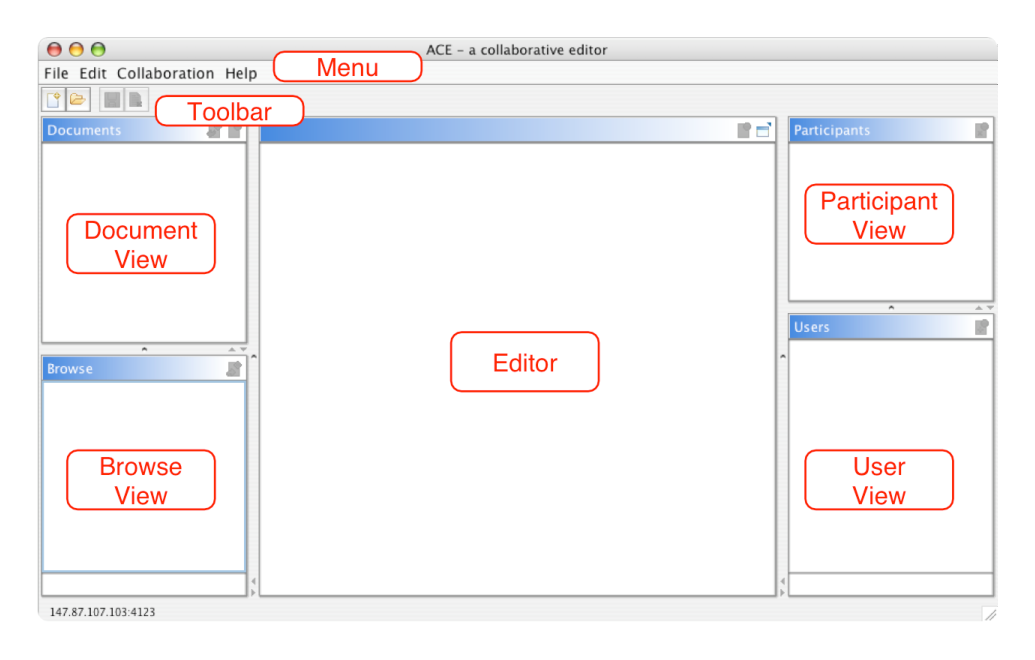
\includegraphics[height=3.135in, width=5.01in]{../images/usermanual/g_ace_overview.eps}
\caption{ACE Overview}
\label{ace_overview}
\end{center}
\end{figure}

% 3.1 MENUS
\subsection{Menu}
The menus (see figure \ref{ace_overview}) are needed to operate the editor. Each menu entry contains multiple functions (actions) which you can use with a simple mouse click. There are four menu entries:
\begin{itemize}
\item File Menu: Use this menu to do the basic editor functions like create new, open and save documents, change your preferences and quit the application. See section \ref{first_steps} for a more detailed description of those functions.
\item Edit Menu: Use this menu for text functions like cut, copy, paste \& select all.
\item Collaboration Menu: This menu is used for all collaborative functions described in section \ref{sect_networking}.
\item Help Menu: This menu contains some additional entries. For example you can open the about box which gives you information about the version of ACE you are using.
\end{itemize}

% 3.2 TOOLBAR
\subsection{Toolbar}
The toolbar (see figure \ref{ace_overview}) contains the most used functions which are not placed on other visible GUI components (except in the menu).
\begin{figure}[H]
\begin{center}
  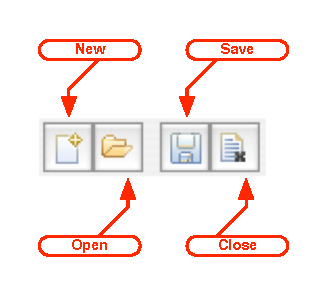
\includegraphics[height=1.74in, width=1.96in]{../images/usermanual/g_toolbar.eps}
\caption{ACE Toolbar}
\label{ace_toolbar}
\end{center}
\end{figure}

% 3.3 EDITOR
\subsection{Editor}
The editor (see figure \ref{ace_overview}) is the main component of ACE. It displays the text of your documents. There is a simple but very usefull feature to gain more writing space. Press the button (marked red in the figures below) or double click with your mouse on the editor title (top bar of the editor) to toggle between normal and full screen editing mode.

\begin{figure}[H]
\begin{center}
  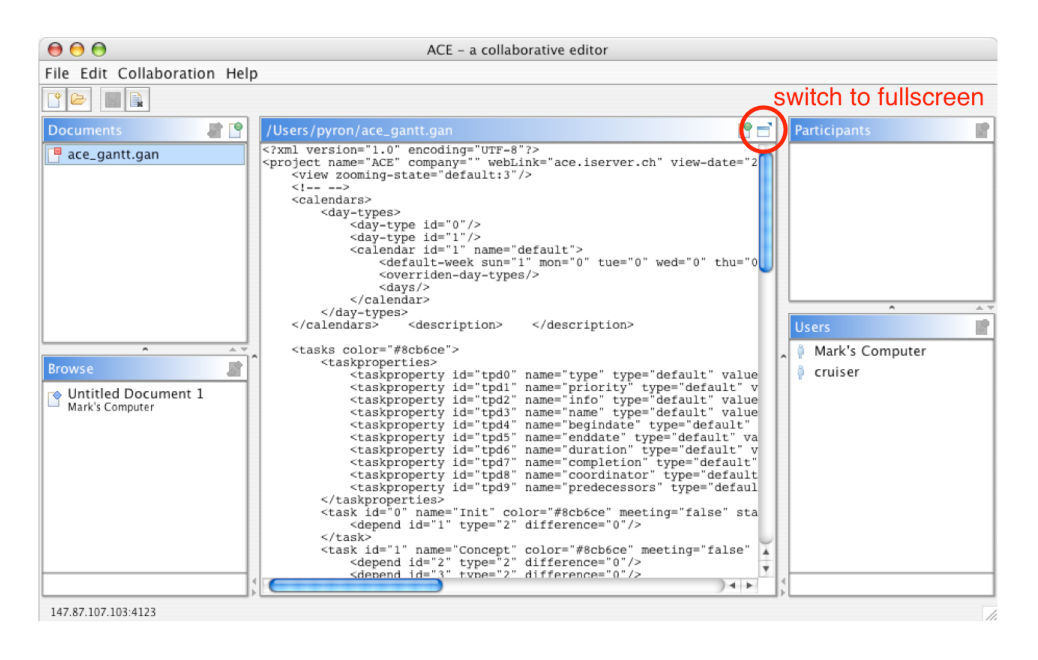
\includegraphics[height=2.09in, width=3.34in]{../images/usermanual/g_editor_normalscreen.eps}
\caption{ACE in normal editing view}
\label{ace_editor_normal}
\end{center}
\end{figure}

\begin{figure}[H]
\begin{center}
  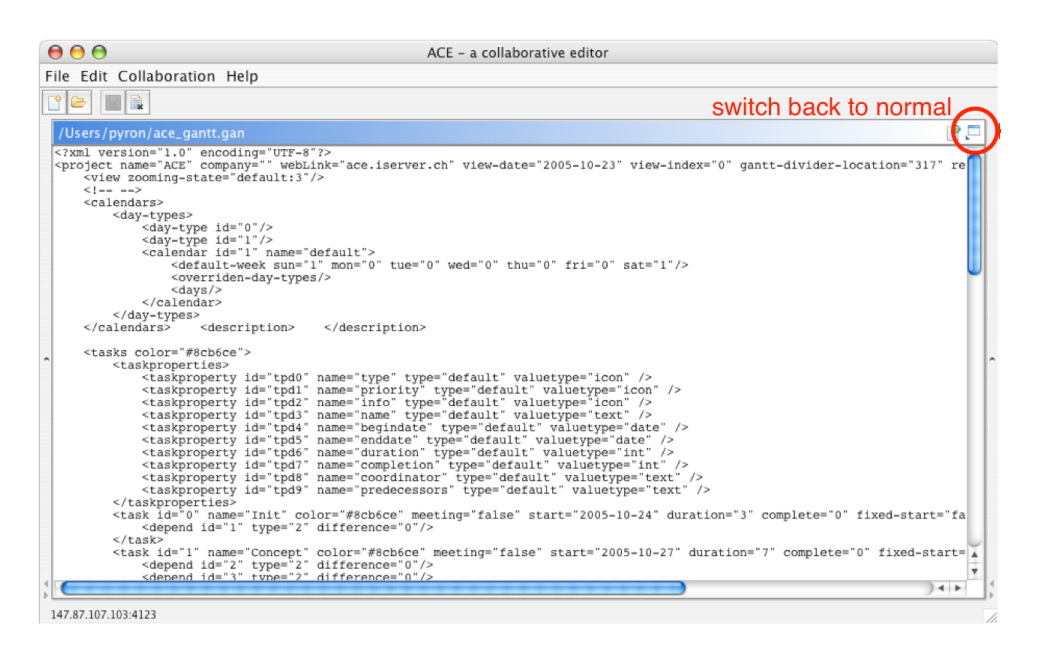
\includegraphics[height= 2.09in, width=3.34in]{../images/usermanual/g_editor_fullscreen.eps}
\caption{ACE in fullscreen editing view}
\label{ace_editor_full}
\end{center}
\end{figure}

% 3.4 VIEWS
\subsection{Views}
This sections explains the four views ACE is using. The document view helps you to manage your open documents. The user view displays all other users running ACE in your network. The browse view shows their documents and if you are writing with other users in the same document you see all the participants in the participant view. \\
\\
Moreover each view has an own toolbar which is placed at the right side in the top border. This toolbar contains the most used functions correspnding to the view.


% 3.4.1 DOCUMENT VIEW
\subsubsection{Document View}
The \textit{Document View} shows all your currently open documents. Basically there are two different document types. \textit{Local documents} are documents on your local machine. ACE provides you the standard editor functionalities as create new, open, save and close local documents. Further, you can publish (see \ref{publish_conceal_documents}) your local documents to make it accessible for other users. \textit{Joined documents} are documents published by other users over the network which you joined. See \ref{join_leave_documents} for more informations about joining documents. \\

\begin{figure}[H]
\begin{center}
  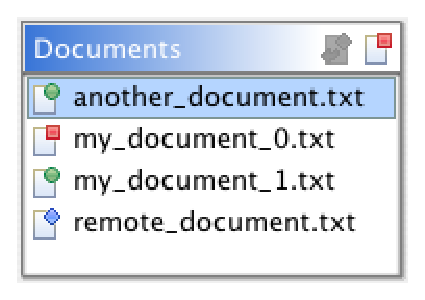
\includegraphics[height=0.89in, width=1.31in]{../images/usermanual/dview_overview.eps}
\caption{Document View}
\label{view_document}
\end{center}
\end{figure}

Different images for each document type makes them well distinguishable (from left to right: local, published \& remote icon):

\begin{figure}[H]
\begin{center}
  
\includegraphics[height=32pt, width=32pt]{../images/usermanual/icon_local.eps}
\vspace{24pt}
  
\includegraphics[height=32pt, width=32pt]{../images/usermanual/icon_published.eps}
\vspace{24pt}
  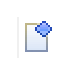
\includegraphics[height=32pt, width=32pt]{../images/usermanual/icon_remote.eps}
\caption{Document Icons}
\label{default}
\end{center}
\end{figure}

% 3.4.2 USER VIEW
\subsubsection{User View}
The \textit{User View} shows all other users currently using ACE in your network. This is used to invite (see section \ref{invite_kick_users}) other users to your published documents. \\

\begin{figure}[H]
\begin{center}
  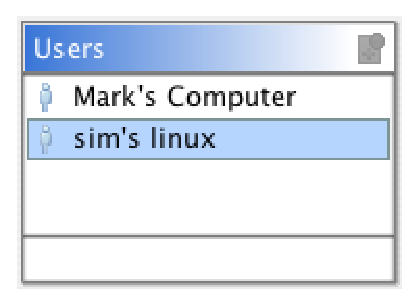
\includegraphics[height=0.91in, width=1.28in]{../images/usermanual/uview_overview.eps}
\caption{User View}
\label{view_user}
\end{center}
\end{figure}

To avoid a complex list with usernames you can use the user view filter. Typing full usernames or parts of it into the textfield below excludes all users not matching.

\begin{figure}[H]
\begin{center}
  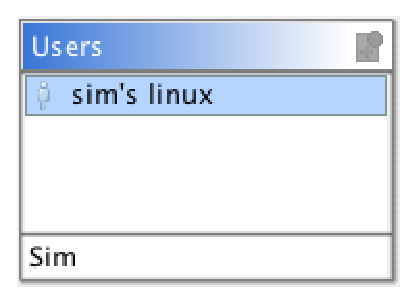
\includegraphics[height=0.9in, width=1.28in]{../images/usermanual/uview_filtering.eps}
\caption{User View Filtering}
\label{view_user_filter}
\end{center}
\end{figure}

% 3.4.3 BROWSE VIEW
\subsubsection{Browse View}
The \textit{Browse View} contains a list with all published documents that can be found in a network. Each list entry contains the document title and the name of the publisher. You need this list to join (see section \ref{join_leave_documents}) published documents.

\begin{figure}[H]
\begin{center}
  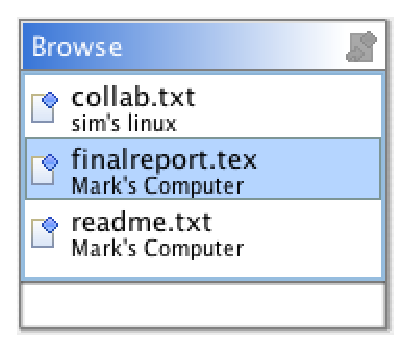
\includegraphics[height=1.06in, width=1.25in]{../images/usermanual/bview_overview.eps}
\caption{Browse View}
\label{view_browse}
\end{center}
\end{figure}

The filtering function helps you to find documents from a specified user. Simple type fragments of the username your are looking for into the text field at the bottom of the view.

\begin{figure}[H]
\begin{center}
  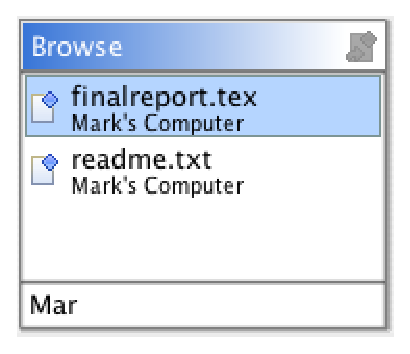
\includegraphics[height=1.07in, width=1.25in]{../images/usermanual/bview_filtering.eps}
\caption{Browse View Filtering}
\label{view_browse_filter}
\end{center}
\end{figure}

% 3.4.4 PARTICIPANT VIEW
\subsubsection{Participant View}
When you publish or join a network document you can see a list of all participants in the \textit{Participant View}. Each participant has his own color which is showed on the right side of his username. This colors are used to highlight the text and to draw the cursor or selection from the corresponding participant. If you are the owner of the document you can select a participant and kick (see section \ref{invite_kick_users}) him from the current document.

\begin{figure}[H]
\begin{center}
  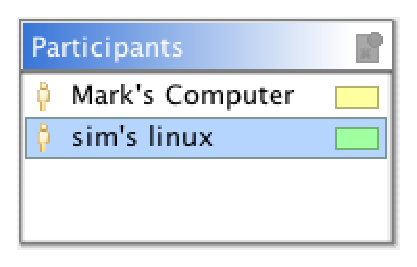
\includegraphics[height=0.78in, width=1.28in]{../images/usermanual/pview_overview.eps}
\caption{Participant View}
\label{view_participant}
\end{center}
\end{figure}


% 3.6 PREFERENCES
\subsection{Preferences}
The preference dialog can be found in the file menu. You need it to change you current settings like your user name, the font size or encoding. The encoding is only used to load and save documents. Default is ISO-8859-1.

\begin{figure}[H]
\begin{center}
  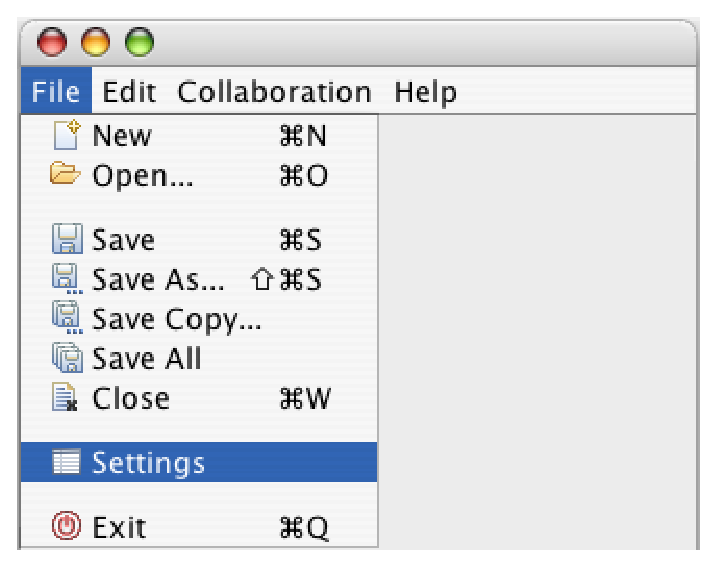
\includegraphics[height=1.78in, width=2.28in]{../images/usermanual/menu_file_preferences.eps}
\caption{Preferences Menu}
\label{view_preferences_menu}
\end{center}
\end{figure}

\begin{figure}[H]
\begin{center}
  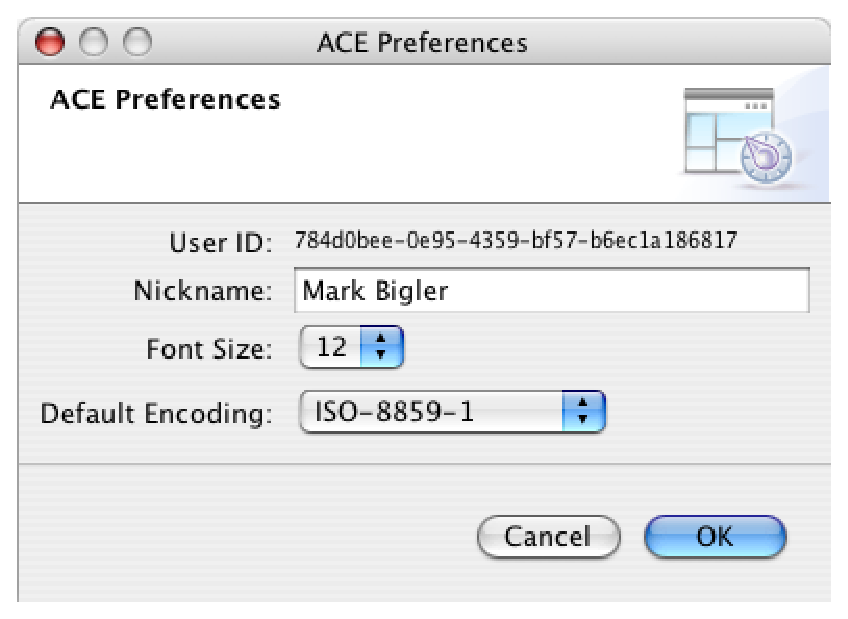
\includegraphics[height=1.95in, width=2.71in]{../images/usermanual/ace_preferences.eps}
\caption{Preferences Dialog}
\label{view_preferences_dialog}
\end{center}
\end{figure}

% 3.7 ABOUT
\subsection{About}
The about dialog shows you the version number of your current used ACE. You can find the about dialog in the menu \textit{help}.
\begin{figure}[H]
\begin{center}
  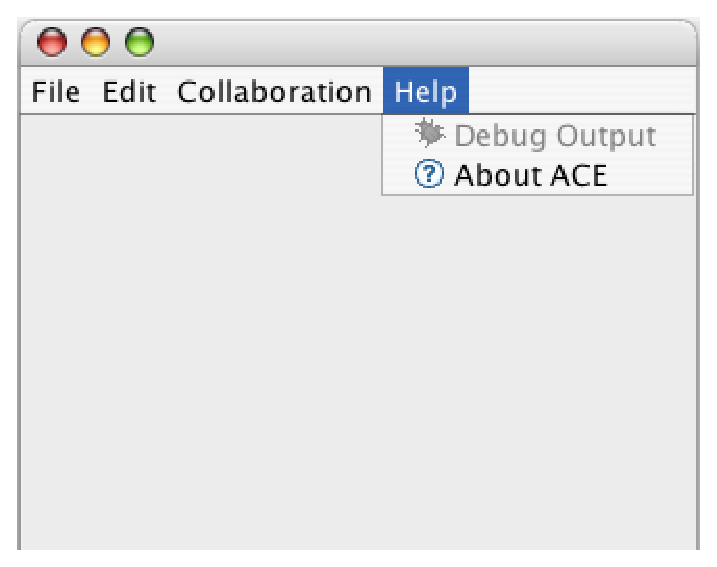
\includegraphics[height=1.78in, width=2.28in]{../images/usermanual/menu_help.eps}
\caption{About Menu}
\label{menu_about}
\end{center}
\end{figure}

\begin{figure}[H]
\begin{center}
  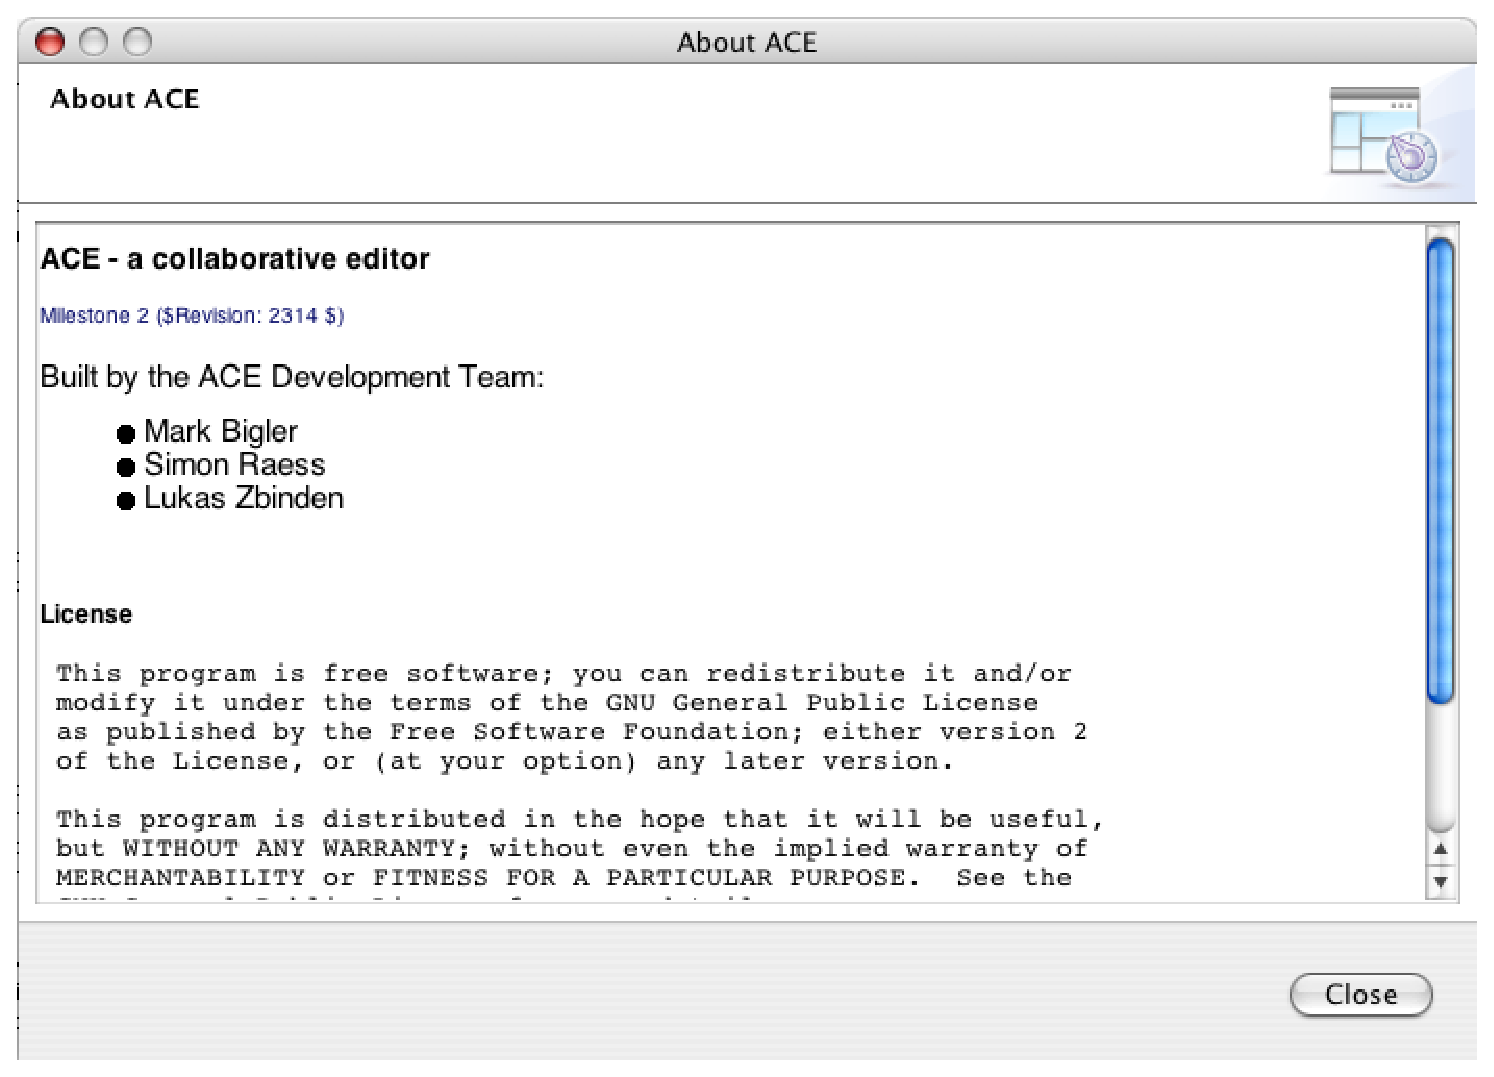
\includegraphics[height=1.47in, width=2.39in]{../images/usermanual/ace_about.eps}
\caption{About Dialog}
\label{dialog_about}
\end{center}
\end{figure}



\newpage
% 4. FIRST STEPS
\section{First Steps}
\label{first_steps}

% 4.1 CREATE
\subsection{Create a new Document}
First of all, you need to create a new document to start writing text. There are three different ways to create a new document:
\begin{itemize}
\item The most comon way to create a new document is by clicking on \textit{new document} on the \textbf{toolbar}.
\item You can also create new document by using the \textbf{menu} (File -> New) or
\item by using the \textbf{shortcut} \textit{CTRL+N}.
\end{itemize}

After you created a new document it appears in the \textit{Document View} on upper left side of your editor.

% 4.2 OPEN
\subsection{Open an existing Document}
To open a existing document you have three posibilites:
\begin{itemize}
\item \textit{open document} on the \textbf{toolbar}.
\item You can also open documents by using the \textbf{menu} (File -> Open) or
\item by using the \textbf{shortcut} \textit{CTRL+O}.
\end{itemize}

% 4.3 SAVE
\subsection{Save open Documents}

To save a open document that have been changed you have three posibilites:
\begin{itemize}
\item \textit{save document} on the \textbf{toolbar}.
\item You can also save documents by using the \textbf{menu} (File -> Save) or
\item by using the \textbf{shortcut} \textit{CTRL+S}.
\end{itemize}

If you save a document the first time then a save dialog will displayed where you can enter a document name.

% 4.4 QUIT
\subsection{Quit}
This dialog appears when you want to quit the application while you have unsaved documents. You can choose between four actions:
\begin{itemize}
\item Cancel: Closes the dialog without doing anything. Also stops the terminate process and doesnt exit the application.
\item Save All: Save's all listed documents. You will be asked for each document to enter a document name if the document hasnt allready one.
\item Save None: Save's none of the listed documents and quits the application.
\item Save Selected: Save's only the selected files and quits the application. If a file hasnt allready a name you will be asked to enter a document name.
\end{itemize}

\begin{figure}[H]
\begin{center}
  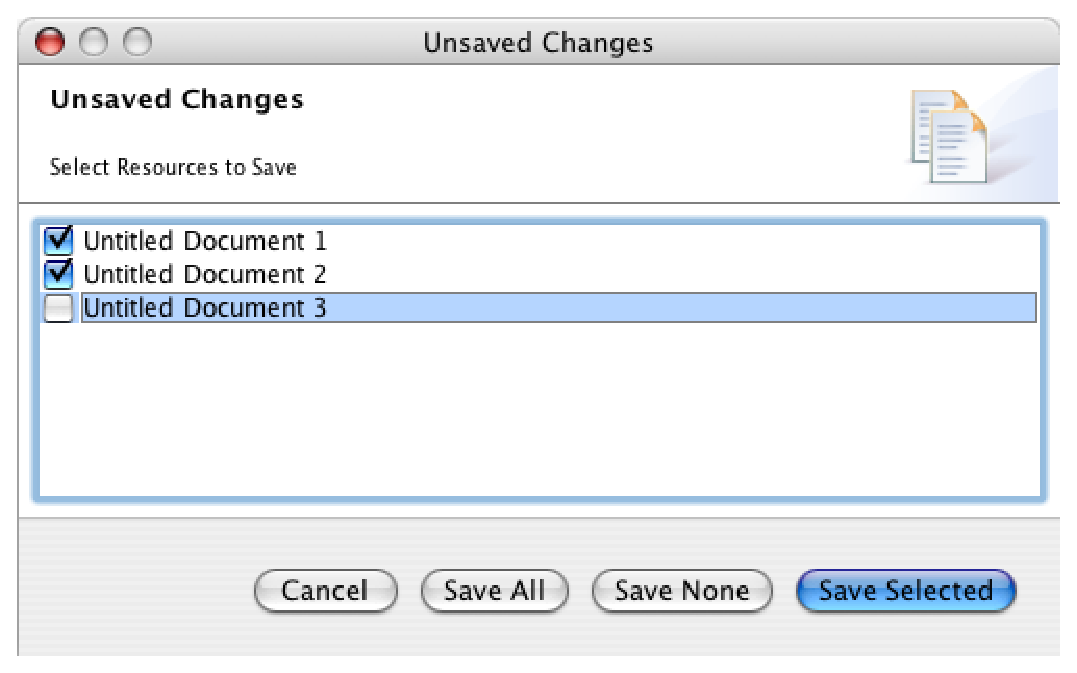
\includegraphics[height=3.20in, width=5.22in]{../images/usermanual/ace_savedialog.eps}
\caption{Save Dialog}
\label{dialog_quit_save}
\end{center}
\end{figure}




\newpage
% 5. NETWORKING
\section{Networking}
\label{sect_networking}

% 5.1 PUBLISH / CONCEAL
\subsection{Publish Documents}
\label{publish_conceal_documents}
Publishing documents is one of the features making ACE to a collaborative editor. This is allways the first step to edit documents with other users. Eighter you publish a document and invite other users or you publish a document and others users are joining it themself. \\
\\
NOTE: only published documents can be viewed by other users!\\

\begin{figure}[H]
\begin{center}
  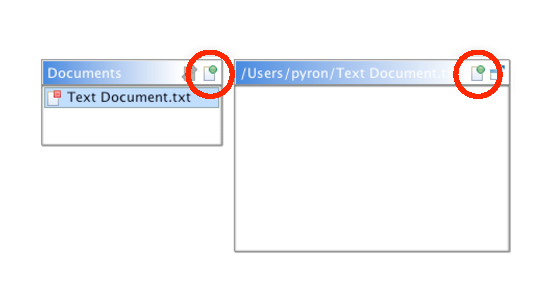
\includegraphics[height=1.32in, width=3.16in]{../images/usermanual/g_editor_view_publish.eps}
\caption{Publish Document}
\label{editor_view_publish}
\end{center}
\end{figure}

To publish a document you first need to select the document in the document view. After you selected the document, eighter click the button on the top of the editor or document view. Advanced users can use the short cut \textit{CTRL+SHIFT+P}.

\begin{figure}[H]
\begin{center}
  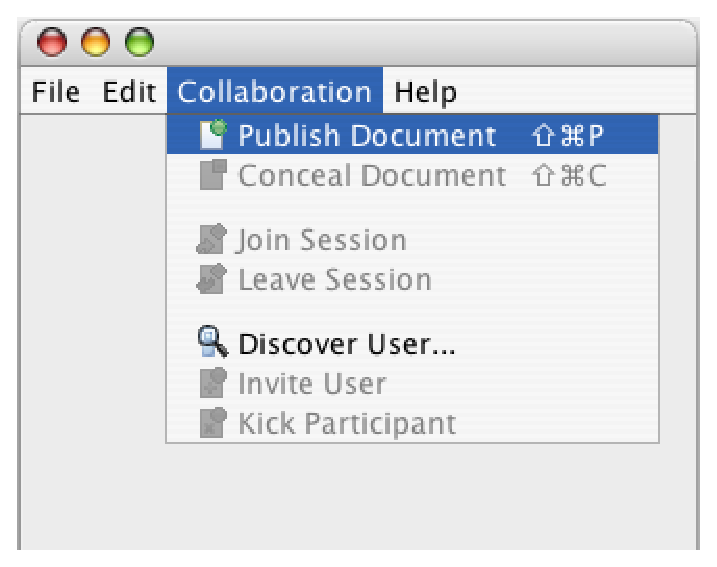
\includegraphics[height=1.78in, width=2.28in]{../images/usermanual/menu_collab_publish.eps}
\caption{Publish Document (Menu)}
\label{menu_publish}
\end{center}
\end{figure}

\subsection{Conceal Documents}
To conceal (unpublish) a document, select it and click on the conceal-button (red marked in the figure below). After a document is conceal, all participants that have been writing in the document receiving a notification that the session is over. They have a local copy of the document in their editor.

\begin{figure}[H]
\begin{center}
  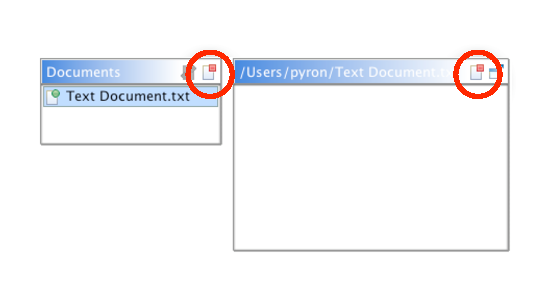
\includegraphics[height=1.32in, width=3.16in]{../images/usermanual/g_editor_view_conceal.eps}
\caption{Conceal Document}
\label{editor_view_conceal}
\end{center}
\end{figure}

You can use the action in the \textit{collaboration menu} to conceal the document or advanced users can use the short cut \textit{CTRL+SHIFT+C}.

\begin{figure}[H]
\begin{center}
  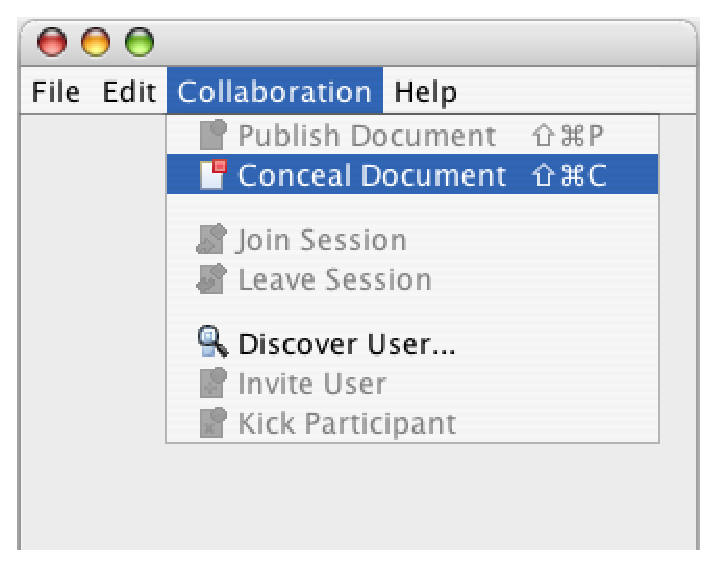
\includegraphics[height=1.78in, width=2.28in]{../images/usermanual/menu_collab_conceal.eps}
\caption{Conceal Document (Menu)}
\label{menu_conceal}
\end{center}
\end{figure}

% 5.2 INVITE / KICK
\subsection{Invite Users}
\label{invite_kick_users}
After you published a document (see section \ref{publish_conceal_documents}) you can invite users. Select the document from the \textit{document view} and the user you want to invite from the \textit{user view}. Eighter click the invite-button on the top border of the user view:

\begin{figure}[H]
\begin{center}
  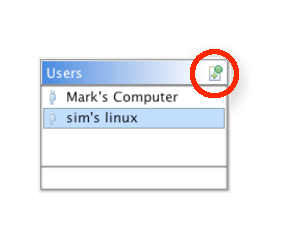
\includegraphics[height=0.78in, width=1.28in]{../images/usermanual/g_uview_invite.eps}
\caption{Invite User}
\label{default}
\end{center}
\end{figure}

or use the action from the \textit{collaboration menu}:

\begin{figure}[H]
\begin{center}
  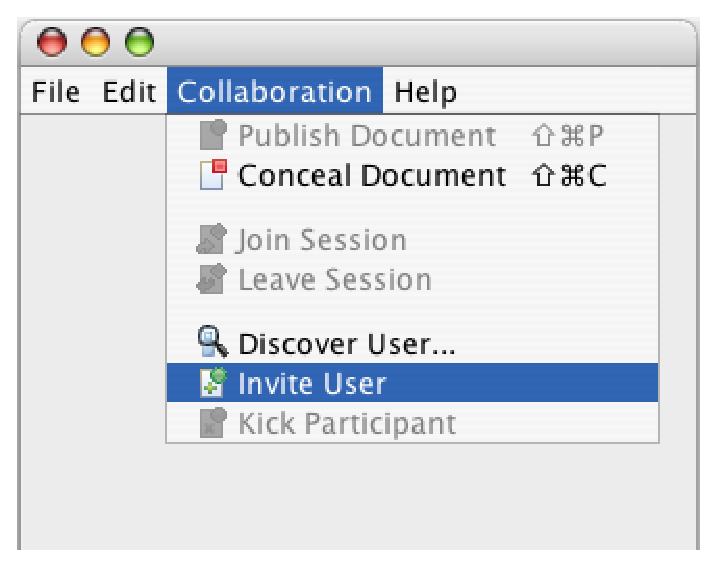
\includegraphics[height=1.78in, width=2.28in]{../images/usermanual/menu_collab_invite.eps}
\caption{Invite User (Menu)}
\label{default}
\end{center}
\end{figure}

\subsection{Kick Users}
The converse operation of inviting is kicking. This function has been added to "remove" bothering participants. Only the publisher of a document can kick users. NOTE: after you kicked a participant, ACE automatically puts him to a blacklist what means that he cant join (see section \ref{join_leave_documents} for more details about joining) the same document again.

\begin{figure}[H]
\begin{center}
  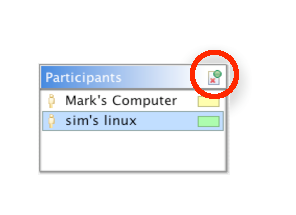
\includegraphics[height=0.78in, width=1.28in]{../images/usermanual/g_pview_kick.eps}
\caption{Kick User}
\label{default}
\end{center}
\end{figure}

Select the published document, the users you want to kick and press the \textit{kick-button} on the top of the \textit{participant view} or use the "Kick Participant" entry from the \textit{collaboration menu}.

\begin{figure}[H]
\begin{center}
  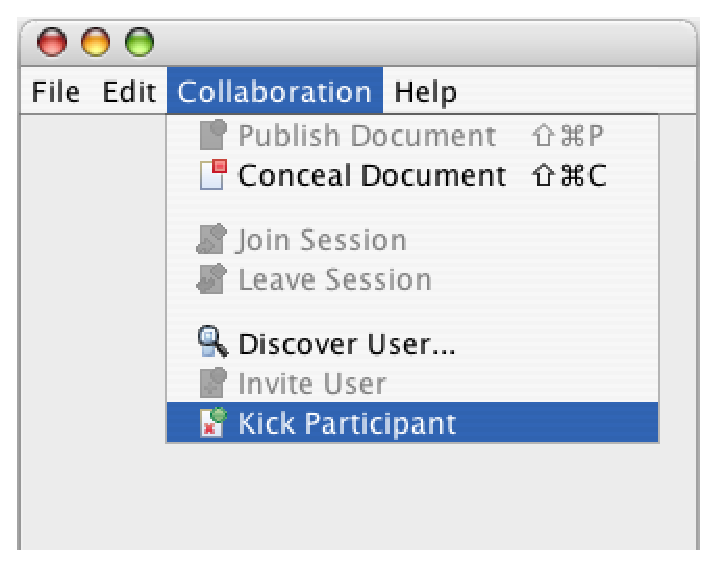
\includegraphics[height=1.78in, width=2.28in]{../images/usermanual/menu_collab_kick.eps}
\caption{Kick User (Menu)}
\label{default}
\end{center}
\end{figure}

% 5.3 JOIN / LEAVE
\subsection{Join Network Documents}
\label{join_leave_documents}
To participate editing in other users documents you need to join such a document. Basically you can join all the documents that are listed in the \textit{browse view}. Select the corresponding document and press the join-button, click on the "Join Session" in the menu or simple double click on it.

\begin{figure}[H]
\begin{center}
  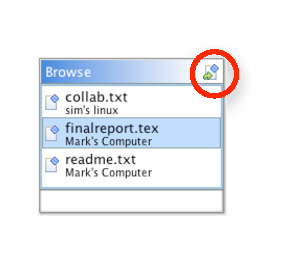
\includegraphics[height=1.56in, width=2.56in]{../images/usermanual/g_bview_join.eps}
\caption{Join Document}
\label{default}
\end{center}
\end{figure}

\begin{figure}[H]
\begin{center}
  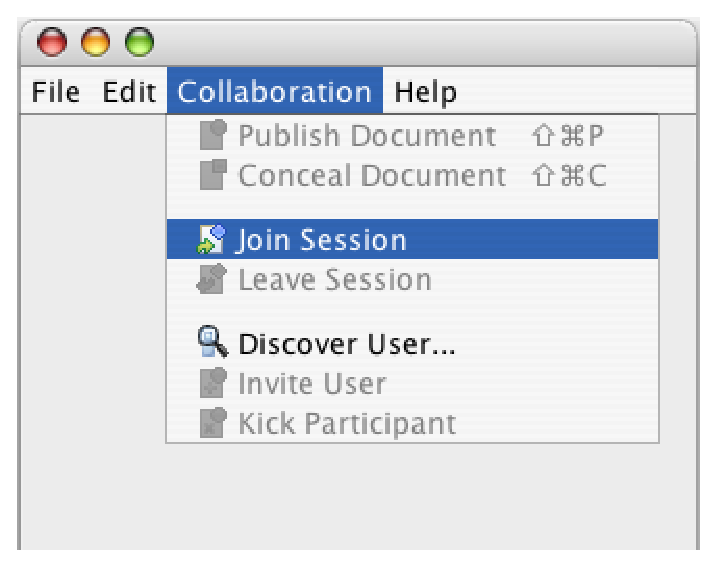
\includegraphics[height=1.78in, width=2.28in]{../images/usermanual/menu_collab_join.eps}
\caption{Join Document (Menu)}
\label{default}
\end{center}
\end{figure}

After you started this joining process the publisher (owner) receives a notification and he can "accept" or "deny" your join request. If he accept's your join request you become a participant and you can start writing your text into the document. See section \ref{collaborative_editing} for more details about collaborative editing.

\subsection{Leave Network Documents}
If you dont want to participate longer do a document, you can leave it. Select the document in the \textit{document view} and press the leave button or use the menu entry "Leave Session". You can also close the document which automatically leaves the session too.
\begin{figure}[H]
\begin{center}
  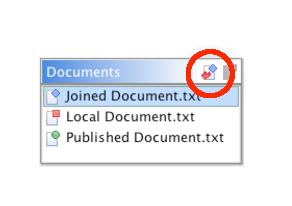
\includegraphics[height=1.56in, width=2.56in]{../images/usermanual/g_dview_leave.eps}
\caption{Leave Document}
\label{default}
\end{center}
\end{figure}

\begin{figure}[H]
\begin{center}
  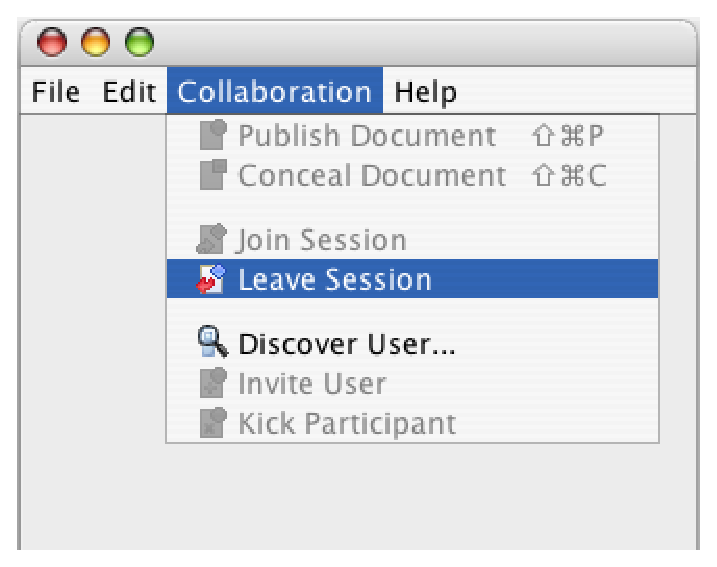
\includegraphics[height=1.78in, width=2.28in]{../images/usermanual/menu_collab_leave.eps}
\caption{Leave Document (Menu)}
\label{default}
\end{center}
\end{figure}


% 5.4 DISCOVER
\subsection{Discover Users}
ACE automatically detects all other users in the same network (subnet). If you want to invite peoples from other networks (e.g. from another company or over the internet) you must explicit discover them. Click in the "Discover User" entry in the collaboration menu. This will open you the dialog shown in figure \ref{discover_dialog}.

\begin{figure}[H]
\begin{center}
  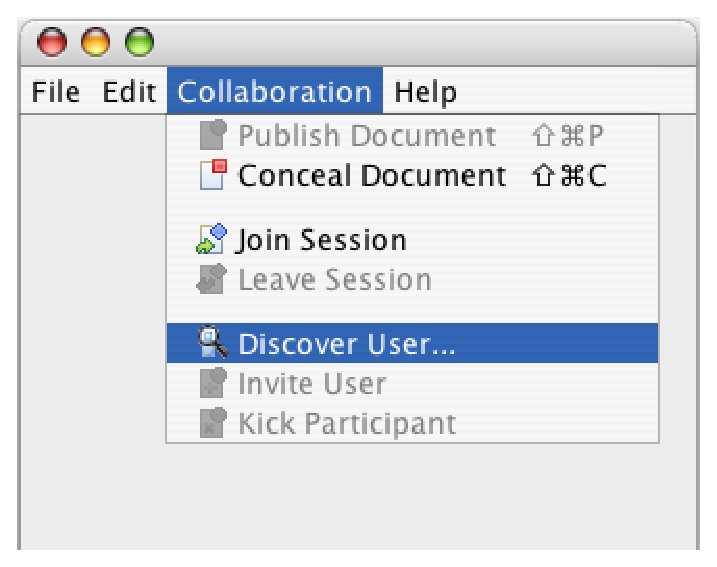
\includegraphics[height=1.78in, width=2.28in]{../images/usermanual/menu_collab_discover.eps}
\caption{Discover User Menu}
\end{center}
\end{figure}

Enter the IP address of the user you want to discover and press ok. Your actual IP address is shown at the bottom of ACE all the time. The other user needs to give you his IP and you can discover him then.

\begin{figure}[H]
\begin{center}
  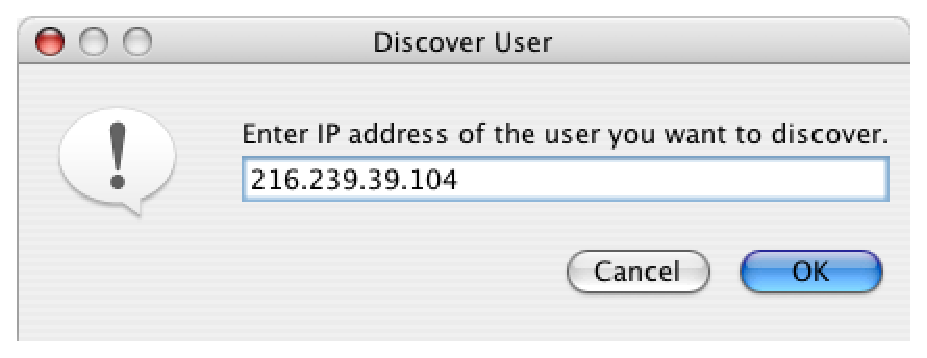
\includegraphics[height=1.08in, width=2.98in]{../images/usermanual/ace_discover.eps}
\caption{Discover User Dialog}
\label{discover_dialog}
\end{center}
\end{figure}

If you enter an invalid IP address the following dialog informs you:

\begin{figure}[H]
\begin{center}
  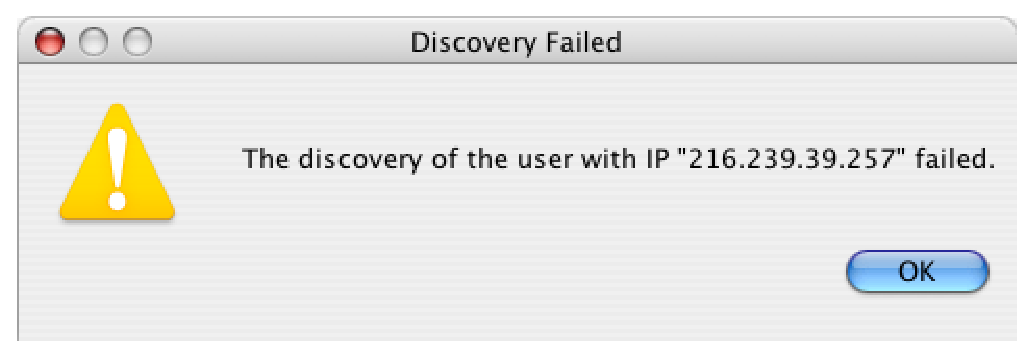
\includegraphics[height=1.08in, width=3.38in]{../images/usermanual/discover_failed_inv_ip.eps}
\caption{Discover Failed Dialog}
\end{center}
\end{figure}

When the IP you entered was valid but there was no ACE running then you receive the following error message:

\begin{figure}[H]
\begin{center}
  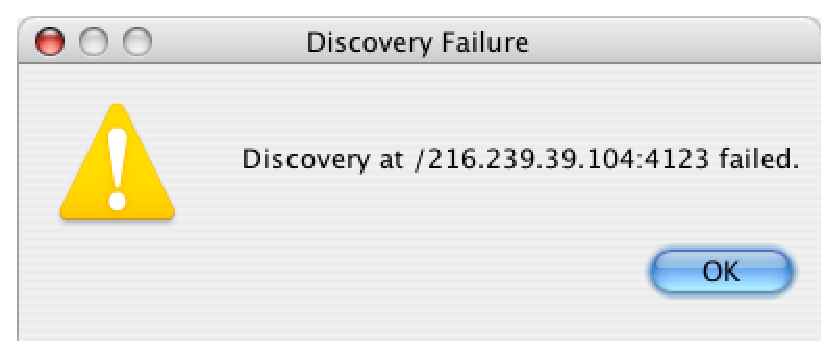
\includegraphics[height= 1.08in, width=2.68in]{../images/usermanual/discover_failed_no_ace.eps}
\caption{Discover Failed Dialog}
\end{center}
\end{figure}

If the discovering was successful the discovered user will be added to the \textit{user view} and you can handle with him.

% COLLAB_EDITING
\subsection{Collaborative Editing}
\label{collaborative_editing}
For each published document you have a participant list. Select the document and the \textit{participant view} will show you the actual list of users participating to this document. Each user (participant) has his own color which is used to highlight the text he wrote:

\begin{figure}[H]
\begin{center}
  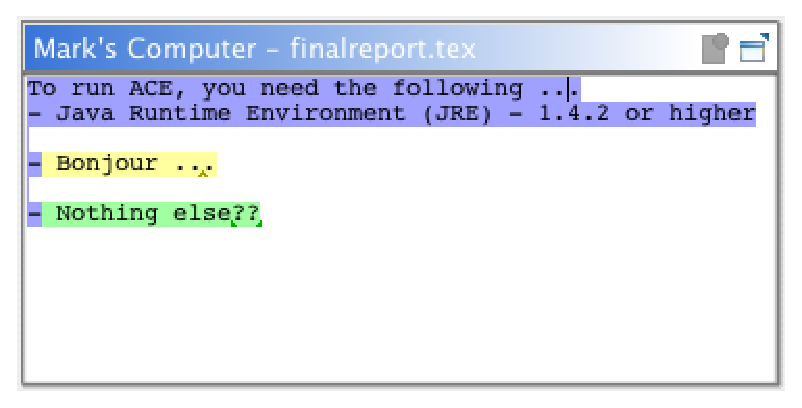
\includegraphics[height=1.25in, width=2.56in]{../images/usermanual/editor_collab_3users.eps}
\caption{Three users in the same document}
\end{center}
\end{figure}

After a participant left (himself or get kicked by the owner), his text will be highlighted grey. In case he joins the document again he will gain back his old color.

\begin{figure}[H]
\begin{center}
  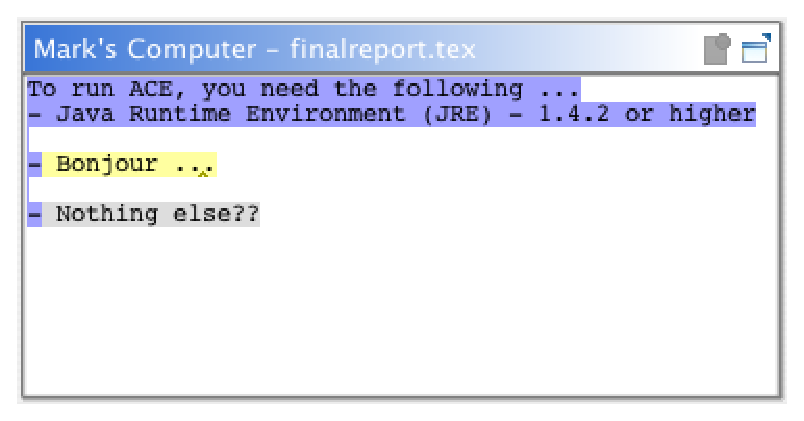
\includegraphics[height=1.29in, width=2.57in]{../images/usermanual/editor_collab_user_left.eps}
\caption{After one user left the document}
\end{center}
\end{figure}


\end{document}
